\documentclass[a4paper]{article}

\usepackage{INTERSPEECH2021}
\usepackage[utf8]{inputenc}
\usepackage[T2A]{fontenc}
\usepackage{caption}
\usepackage{subcaption}

\title{Golos: Russian Dataset for Speech Research}
\name{Nikolay Karpov, Alexander Denisenko, Fedor Minkin}

\address{Sber, Russia}
\email{karpnv@gmail.com, alexander.denisenko@phystech.edu, coauthor@company.com}

\begin{document}

\maketitle
% 
\begin{abstract}
 
This paper introduces Russian speech dataset called Golos, a large corpus suitable for speech research. The dataset mainly consists of audio recorded and manually annotated on the crowd-sourcing platform. Total duration of audio is about 1240 hours. We have made the corpus freely available for downloading, along with acoustic model with CTC loss prepared on this corpus. Additionally transfer learning was applied to improve performance of the acoustic model. In order to evaluate quality with beam-search algorithm we built 3-gram language model on the open Common Crawl dataset. Total word error rate (WER) metrics are about 3.5\% and 11.9\%.


\end{abstract}
\noindent\textbf{Index Terms}: speech recognition, open dataset, Russian language, speech corpus, acoustic model, language model

\section{Introduction}
 We believe that open data is one of the key drivers of recent success in the field of artificial intelligence. In particular automatic speech recognition (ASR) algorithms became much better and more robust during recent years. New algorithms allows to create conversational systems with good user experience so that such technologies become more popular. It creates a basement for many new business ideas, disruptions of traditional strategies and benefits for innovators. 
  
 Despite the existence of outstanding initiatives such as MLS dataset \cite{pratap2020mls} there is a luck of manually annotated large scale speech corpora in Russian that is freely available and suitable for training and testing speech recognition systems.
 
 This article is dedicated to present our new open Russian speech dataset with manual annotation. It can be useful for many research projects which need labeled audio data such as \cite{savchenko2008analyse, gubochkin2013cl}. We provide an example on how to train acoustic model on this data using the open source NeMo toolkit \cite{kuchaiev2019nemo}. We also demonstrate improvement using pre-trained English acoustic models and quality benefits from language model. The highlights of this paper are the following:
\begin{enumerate}
\item Open audio corpus with 1240 hours of manually annotated speech in Russian.\footnote{https://github.com/sberdevices/golos}
\item An example of acoustic model trained on our corpus.
\item Transfer learning empirical results for Russian acoustic model using pre-trained English one.
\item Evaluation of acoustic model on beam-search decoder with language model trained on the open dataset.
\end{enumerate}

Section 2 presents related works that inspired us to share our corpus. In Section 3 we describe the pipeline that we used to build the corpus. Section 4 describes the structure of the dataset. Section 5 presents acoustic model trained on this dataset and experimental results on transfer learning. Finally in Section 6 we provide acoustic model evaluation together with language model, which we also make available.

\section{Related Work}

There are few large scale data collections for speech recognition is available now. 

\subsection{Mono-lingual ASR datasets}

Let us mention only several mono-lingual datasets which we think are most important in the field of Russian speech recognition.

First one is LibriSpeech \cite{panayotov2015librispeech} which includes about 1000 hours of English audio-books. It is derived from the big LibriVox dataset,  distributed under an open license. Second one is an audio part of Wall Street Journal (WSJ) corpus \cite{paul1992design} which contains about 400 hrs. of speech data. These two datasets are usually used to evaluate state of the art (SoTA) speech recognition algorithms.

Open-STT is the only Russian language large-scale dataset. It consists of more then 15000 hours \cite{veysov2020towardimagenetstt}. Unfortunately its annotation is not manually created. Transcriptions are derived by doing  alignment or ASR system. 

\begin{table}[th]
  \caption{Content of Open STT Russian corpus}
  \label{tab:openstt}
  \centering
  \begin{tabular}{ llcr }
    \toprule
    Domain & Annotation & Utterances & Hours~~~  \\
    \midrule
    Radio &     Alignment & 8.3M & 11 996 ~~~  \\
    Public Speech & Alignment  & 1,7M & 2 709 ~~~ \\
    YouTube & Subtitles  & 2,6M & 2 117 ~~~ \\
    Audiobooks & Alignment  & 1,3M & 1 632 ~~~ \\
    Calls & ASR  & 695K & 819 ~~~ \\
    Other & TTS  & 1.9M & 835 ~~~ \\
    \bottomrule
  \end{tabular}
\end{table}

\subsection{Multi-lingual ASR datasets}

We mainly focus on multi-lingual corpuses which include Russian data. VoxForge\footnote{http://www.voxforge.org} may be the oldest and still available open speech resource. It remains a low-scale dataset, which includes about 300 hours in total, and even less in Russian.

CommonVoice \cite{ardila2019common}, is a scalable solution, with more than 30 languages available including Russian, which keeps growing with 4500 (validated) hours currently available.

LibriVox\footnote{https://librivox.org} includes nearly 80 506 hours in total but only 172 hours of Russian audiobooks read by volunteers from around the world.

The M-AILABS\footnote{https://www.caito.de/2019/01/the-m-ailabs-speech-dataset} speech dataset includes data based on LibriVox and Project Gutenberg\footnote{http://www.gutenberg.org}. The data consist of nearly thousand hours of audio in total and 47h hours of Russian speech.

MLS \cite{pratap2020mls} is a large-scale multilingual dataset for speech research like a LibriSpeech and M-AILABS derived from LibriVox dataset and consists of 8 languages, including about 44.5K hours of English and a total of about 6K hours for other languages. However, it doesn't contain any Russian language data.


\section{Data Collection Pipeline}

This section describes the main steps during data collection and preparation. The pipeline is developed to solve a cold start problem when we have a new device but there is no real user data yet. It includes four stages.

\subsection{Templates Creation}
We create a list of domains which is suitable for our products: music, films, organizations, names, addresses, etc.
For each domain we develop so-called templates - structures which let us create highly plausible text queries within certain domain. Basically, it describes the way in which different entities (such as command, movie title, actor name, and specific forms of these entities - including case and gender) might be arranged so that the resulting query might have been a result of some actual use-case. 

For example the template "command + film" can be instantiated as "Switch on Terminator 1"


\subsection{Audio Generation}
Using such templates we consistently generate tens and hundreds of thousands of text queries, which we then proceed to voiceover with real people's voices. We use two type of voice sources: a popular crowd-sourcing platform Yandex.Toloka\footnote{https://toloka.yandex.ru} and studio recordings through our smart screen called SberPortal.

\subsection{Crowd-sourced Validation}
However, we cannot be certain that all the labellers have said exactly what was written in their assignment. We neither want to use such data in train, test or development sets, so we filter them out. We do so by presenting each pair of text and crowdsourced audio-file to 5 people on the very same labelling platform and ask them whether or not the audio matches the text in front of them. If 5 out of 5 people say that it does, then we consider text and audio to match each other. If less than 5 people say so - we don't use this pair at all.

\subsection{Assisted Transcribation}
As our acoustic model is only capable of predicting Cyrillic symbols and spaces, in order to train it we have to convert all the texts into those lacking any Latin symbols, diacritical symbols, numbers, special symbols and so on. In order to do so - we use Toloka again! Labellers are being presented with original text which might contain any symbols whatsoever, corresponding audio which was validated in the previous step and they are asked to transcribe the text with Cyrillic symbols and spaces only. 

For us it turned out to be vital to provide not only audios, but also hints in the form of original text as it might be extremely difficult to transcribe the audio of a Russian who is pronouncing "Annenmaykantereit Barfuß am Klavier"  without any assistance. For each pair of audio and text, we present it to 5 labellers. We take a look at the most common transcription in Cyrillic - and if there are at least two people who have written this exact transcription - we use it as the true label when training our acoustic model.

\section{Dataset Overview}

There are two types of audio sources in our corpus. First one is a crowd-sourcing platform Yandex.Toloka. We call it as a Crowd domain below. Second one is our target source - a smart screen SberPortal. The sales of SberPortal have not started by the development stage. So we have to generate audio through SberPortal in the studio by emulating real user environment. To do it we use 1 meter, 3 meters and 5 meters distances between speaker and device. We call it a Farfield domain below because the distance is usually quite far.

Each of sources we split into training and testing subsets. The testing part of Crowd set consists of about 10K files, Farfield testing set is about 2K. The exact dataset separation is shown in Table~\ref{tab:dataset_separation}. 

\begin{table}[th]
  \caption{Golos Dataset Content Separation.}
  \label{tab:dataset_separation}
  \centering
  \begin{tabular}{ l|r|r|r|r }
    \toprule
    \multicolumn{1}{l|}{\textbf{Domain}} & \multicolumn{2}{c|}{\textbf{Train files and hours}} & \multicolumn{2}{c}{\textbf{Test files and hours}} \\
    \midrule
    Crowd  & 979796 & 1095~~h.  & 9994 & 11.2 h. \\
    Farfield & 124003 & 132.4 h. &  1916 & 1.4 h. \\
    \bottomrule
    Total  & 1103799 & 1227.4 h. & 11910 & 12.6 h. \\
  \end{tabular}
\end{table}

We don't have information about speaker of recordings so the separation done without it. A voice of the same user could appear in training and testing subsets. 


\begin{table}[t]
  \caption{Golos Training Set Description.}
  \label{tab:dataset_description}
  \centering
  \begin{tabular}{lrr}
    \toprule
    \textbf{Description}      & \textbf{Crowd  subset}     & \textbf{Farfield subset} \\
    \midrule
    Count & 979796 files & 124003 files \\
    Mean & 4.0~~ sec. & 3.8 ~~ sec. \\
    STD &  1.9~~ sec. & 1.6 ~~ sec. \\
    Min & 0.02 sec. & 0.002 sec. \\
    25th percentile& 2.8~~ sec. & 2.8 ~~ sec. \\
    50th percentile& 3.7~~ sec. & 3.5 ~~ sec. \\
    75th percentile& 4.8~~ sec. & 4.5 ~~ sec. \\
    Max & 56.3~~ sec. & 23.5 ~~ sec. \\
    \bottomrule
  \end{tabular}
\end{table}

Some statistical data like percentile, mean and standard deviation (STD) of the duration values of the training sets provided in the Table \ref{tab:dataset_description}. Figure \ref{fig:duration_distribution} shows a histogram of the duration distribution of utterances in the training set.

\begin{figure}[ht]
\begin{subfigure}{.49\linewidth}
  \centering
  % include first image
  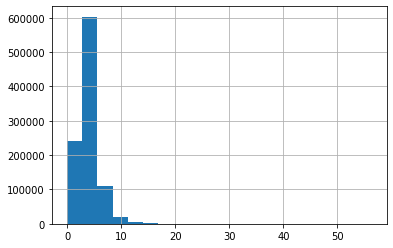
\includegraphics[width=1.\linewidth]{LaTeX/img/toloka_lens.png}  
  \caption{Crowd domain.}
  \label{fig:sub-first}
\end{subfigure}
\begin{subfigure}{.49\linewidth}
  \centering
  % include second image
  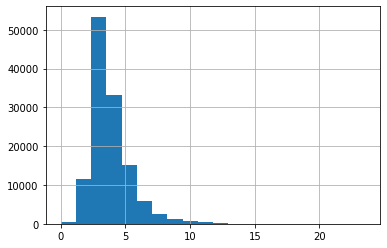
\includegraphics[width=1.\linewidth]{LaTeX/img/portal_lens.png}  
  \caption{Farfield domain.}
  \label{fig:sub-second}
\end{subfigure}
\caption{Number of samples depends on sample duration (sec.) in Golos training set.}
\label{fig:duration_distribution}
\end{figure}

To perform any limited  or  no  supervision experiments with models we provide additional subsets of training set with duration 100 hours, 10 hours, 1 hour, 10 minutes as it was in the previous work \cite{kahn2020libri}.

\section{Acoustic Model}

The best way to show the quality of data is to train some model on it and estimate quality metrics of the model. We estimate word error rate (WER) because it is a common performance metric of the speech recognition system. 

\subsection{Experiment Setup}

As an acoustic model we chose QuartzNet15x5 neural network \cite{kriman2020quartznet} which architecture is shown on the Table \ref{tabular:Quartznet}. The model starts with a convolutional layer $C_1$ followed by a sequence of 5 groups of blocks. Blocks in the group are identical, each block $B_k$ consists of R time-channel separable K-sized convolutional modules with C output channels. Each block is repeated S times. The model has 3 additional conv layers ($C_2, C_3, C_4$) at the end.

The training procedure is done by using the open source NeMo toolkit \cite{kuchaiev2019nemo}. We train our model on the Nvidia DGX-2 with 16 GPU cards Tesla v100 with a batch size of 88 per GPU and accumulate gradients every 10 batches, so our effective batch size is 16*88*10 = 14080. In order to decrease the memory and training time, we used mixed-precision training \cite{micikevicius2017mixed}.

We train an acoustic model on the whole randomly shuffled training part of dataset end evaluate it on two test sets separately (Crowd and Farfield domains). Data augmentation is carried out using SpecAugment \cite{park2019specaugment} without time warping deformation. We don't use dropouts during training. Training is conducted with the help of the NovoGrad \cite{ginsburg2019stochastic} optimizer ($\beta_1$ = 0.95, $\beta_2$ = 0.5) with a cosine annealing learning rate policy. About 5\% steps of learning rate warm-up helps stabilize early training with maximum learning rate of 0.01, and weight decay 0.001. Bigger learning rate leads to gradient overflow and infinite loss value in our experiments. 

\begin{table}[t]
  \caption{QuartzNet15x5 Architecture with outputs for Russian letters. }
  \label{tabular:Quartznet}
  \centering
  \begin{tabular}{ccccc}
    \toprule
    \textbf{Block}  & \textbf{R} & \textbf{K} & \textbf{C} & \textbf{S}     \\
    \midrule
    $C_1$  & 1 & 33 & 256 &  1  \\
    \midrule
    $B_1$  & 5 & 33 & 256 &  3  \\
    $B_2$  & 5 & 39 & 256 &  3  \\
    $B_3$  & 5 & 51 & 512 &  3  \\
    $B_4$  & 5 & 63 & 512 &  3  \\
    $B_5$  & 5 & 75 & 512 &  3  \\
    \midrule
    $C_2$  & 1 & 87 & 512 &  1  \\
    $C_3$  & 1 & 1 & 1024 &  1  \\
    $C_4$  & 1 & 1 & 34 &  1    \\
    \bottomrule
    \textbf{Params,M}  &  &  & &  18.9     \\
  \end{tabular}
\end{table}


\subsection{Transfer Learning}

Transfer learning is a key element for the recent success of neural networks, so it is widely used in the industry. For example, ImageNet dataset is often utilized for creating pre-trained models in computer vision, and in the natural language processing fields pre-trained Bert models are usually used. 

QuartzNet15x5 acoustic model pre-trained on the 3300 hours of public data in English is publicly available. Russian version of this model is shown on the Table \ref{tabular:Quartznet}. The only difference from the English version is in the last layer as the target language has a different alphabet. For Cyrillic alphabet, there are 34 possible outputs - 32 letters (excluding letter ё), whitespace and blank symbols. When training the model using the Latin alphabet, there are 29 possible outputs - 26 letters, whitespace, blank and apostrophe symbols. Our transfer learning pipeline is as follows:
\begin{itemize}
    \item Take layers weights $C_1, B_1, B_2, B_3, B_4, B_5, C_2, C_3$ from pre-trained network as is and initialize new network with them.
    \item Map similar character (for instance "k"  to "к" ) weights from old $C_4$ layer to the new one.
    \item Randomly initialize weights for new characters in the layer $C_4$
    \item Train the resulting network on a target dataset starting with the same learning rate that was used to pre-train the model from scratch.
\end{itemize}

Figures \ref{fig:crowd_domain} and \ref{fig:portal_domain} demonstrate how our transfer learning procedure affects greedy WER along a training process. There are four training setups: 10 000 steps with random initialization (Green - 10K from scratch), 10 000 steps with English initialization (Red - 10K from En), 20 000 steps with random initialization (Blue - 20K from scratch), 20 000 steps with English initialization (Violet - 20K from En). Each of the training setups has two evaluation sets - Crowd and Farfield - so we have eight curves. We can see that random initialization curves are positioned much higher than initialisation by English model. It means that transfer learning always boosts our performance.

\begin{figure}[ht]
\begin{subfigure}{.99\linewidth}
  \centering
  % include first image
  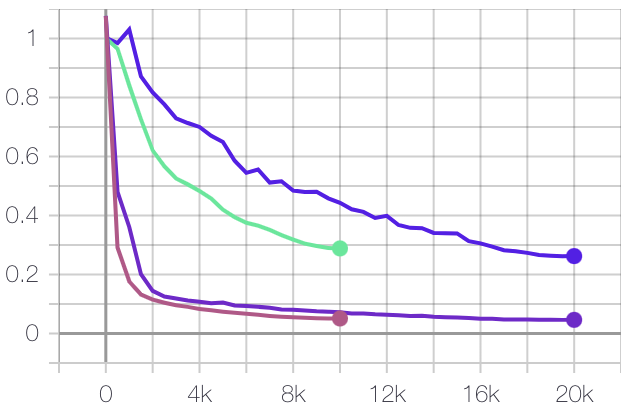
\includegraphics[width=1.\linewidth]{LaTeX/img/crowd10k20k.png}  
  \caption{Crowd domain.}
  \label{fig:crowd_domain}
\end{subfigure}
\begin{subfigure}{.99\linewidth}
  \centering
  % include second image
  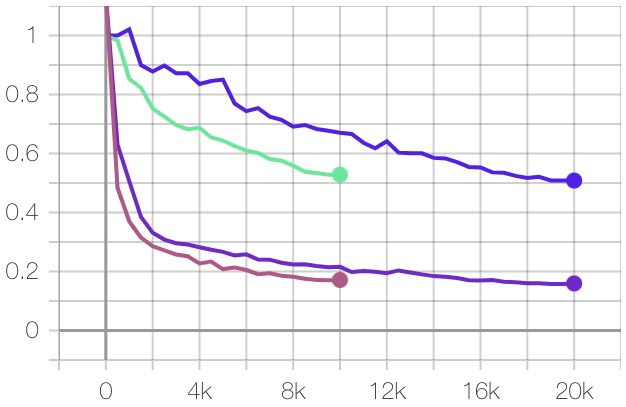
\includegraphics[width=1.\linewidth]{LaTeX/img/portal10k20k.png}  
  \caption{Farfield domain.}
  \label{fig:portal_domain}
\end{subfigure}
\caption{Greedy WER dependence on transfer learning. Green - 10K from scratch, Blue - 20K from scratch. Red - 10K from En, Violet - 20K from En.}
\label{fig:portal_crowd_domain}
\end{figure}

Table \ref{tab:wer_50k} shows a final values of greedy WER for our domains. There are three experiments with different training durations. 50 000 steps took about 8 days long, 20 000 steps took 2 days 21 hours, 10 000 steps took 1 day 19 hours. These WER scores have been calculated using the greedy decoder. The best values are 4.327\% and 15.28\% on the Crowd and Farfield domain respectively and were shown by the model which was trained for 50K steps. 

\begin{table}[t]
  \caption{Transfer Learning Influence.}
  \label{tab:wer_50k}
  \centering
  \begin{tabular}{lrr}
    \toprule
    \textbf{Training procedure } & \textbf{Crowd} & \textbf{Farfield} \\
    \midrule
    10K from scratch   &  28.84\%   & 52.82\% \\
    10K from En.    & 5.095\%       & 17.13\%  \\
    \midrule
    20K from scratch   &  26.24\%   & 50.82\% \\
    20K from En.    & 4.629\%       & 15.95\% \\
    \midrule
    50K from En.    & 4.327\%       & 15.28\% \\
    \bottomrule
  \end{tabular}
\end{table}


Figure \ref{fig:wer_steps} demonstrates how greedy WER is changing along the whole training process for three training setups initialized by the pre-trained English model. 

\begin{figure}[ht]
\begin{subfigure}{.49\linewidth}
  \centering
  % include first image
  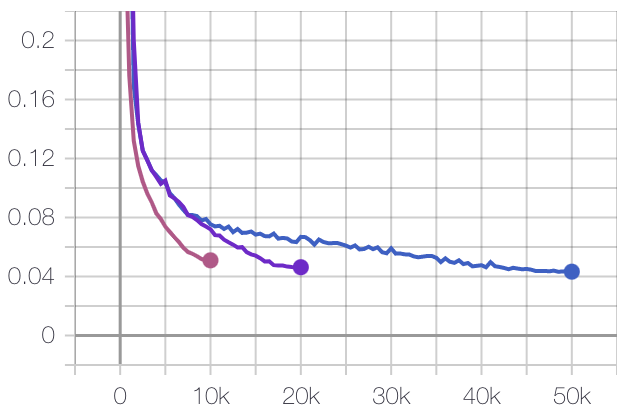
\includegraphics[width=1.\linewidth]{LaTeX/img/crowd_5.095_4.629_4.327_en.png}  
  \caption{Crowd domain.}
  \label{fig:wer_steps1}
\end{subfigure}
\begin{subfigure}{.49\linewidth}
  \centering
  % include second image
  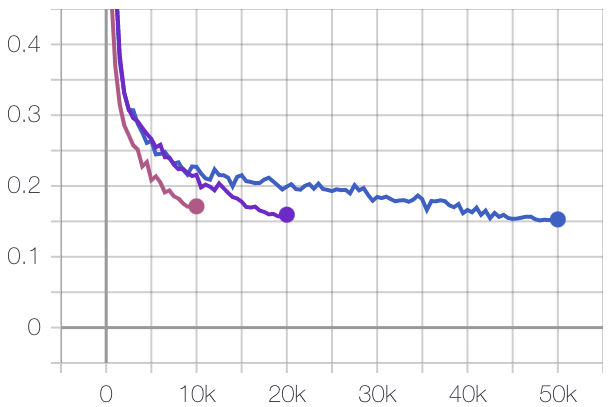
\includegraphics[width=1.\linewidth]{LaTeX/img/portal_17.13_15.95_15.28_en.png}  
  \caption{Farfield domain.}
  \label{fig:wer_steps2}
\end{subfigure}
\caption{Greedy WER (\%) depends on the training duration with English initialisation. Red - 10K, Violet - 20K, Blue - 50K. }
\label{fig:wer_steps}
\end{figure}

\section{Language Model}

We create a language model using the Russian part of the Common Crawl dataset\footnote{https://commoncrawl.org} and KenLM Language Model Toolkit \cite{heafield-2011-kenlm}. The Common Crawl is a repository of web crawl data that can be accessed and analyzed by anyone. KenLM toolkit allows us to create a very fast n-gram language model.

We have created three external 3-gram language models. First one isn using cleaned texts from Common Crawl dataset (CC LM). Second one was built with the help of transcription of training set audios (train LM). Third model is a merge of these two 3-gram models with 50/50 percent weights (CC + train LM).

\begin{table}[t]
  \caption{Common Crawl (CC) Language Model Influence}
  \label{tab:language_model}
  \centering
  \begin{tabular}{lrr}
    \toprule
    \textbf{Model}      & \textbf{Crowd}     & \textbf{Farfield} \\
    \midrule
    20K greedy & 4.629\% & 15.95\%    \\
    20K with CC LM & 4.856\% & 12.57\%   \\
    20K with train LM & 3.661\% & 12.83\%   \\
    20K with CC + train LM & 3.455\% & 11.86\%   \\
    
    \midrule
    50K greedy & 4.327\% & 15.28\%   \\
    50K with CC LM & 4.869\% & 12.59\%   \\
    50K with train LM & 3.784\% & 12.70\%   \\
    50K with CC + train LM & 3.592\% & 11.93\%   \\
    \bottomrule
  \end{tabular}
\end{table}

We use these created language models for inference with beam-search decoder (beam size=16, alpha=2, beta=1.5). Table \ref{tab:language_model} shows how beam-search decoder with our three language models influences the resulting WER. The best WER values with the language model are 3.455\% and 11.86\%. 


\section{Conclusions}

In this paper we reveal an open Russian language dataset. It is a large corpus suitable for speech research. It consists of audios obtained both from the crowd-sourcing platform and from the studio with far field settings. All 1240 hours of audios are manually annotated.

Using our new corpus we have trained a QuartzNet acoustic model with CTC loss. The best performance of the acoustic-model was achieved with the help of transfer learning from pre-trained model on English language. 

Additionally, we built 3-gram language model on the open Common Crawl dataset and merged it with train set transcriptions. Using a beam-search algorithm, our resulting model achieves 3.5\% and 11.9\% WER values on Crowd and Farfield datasets respectively.

All the data and models are freely available for downloading at the Github repository\footnote{https://github.com/sberdevices/golos}.


\section{Acknowledgements}

The authors would like to thank Sber corporation for the funding of this work.

\bibliographystyle{IEEEtran}

\bibliography{mybib}

% \begin{thebibliography}{9}
% \bibitem[1]{Davis80-COP}
%   S.\ B.\ Davis and P.\ Mermelstein,
%   ``Comparison of parametric representation for monosyllabic word recognition in continuously spoken sentences,''
%   \textit{IEEE Transactions on Acoustics, Speech and Signal Processing}, vol.~28, no.~4, pp.~357--366, 1980.
% \bibitem[2]{Rabiner89-ATO}
%   L.\ R.\ Rabiner,
%   ``A tutorial on hidden Markov models and selected applications in speech recognition,''
%   \textit{Proceedings of the IEEE}, vol.~77, no.~2, pp.~257-286, 1989.
% \bibitem[3]{Hastie09-TEO}
%   T.\ Hastie, R.\ Tibshirani, and J.\ Friedman,
%   \textit{The Elements of Statistical Learning -- Data Mining, Inference, and Prediction}.
%   New York: Springer, 2009.
% \bibitem[4]{YourName17-XXX}
%   F.\ Lastname1, F.\ Lastname2, and F.\ Lastname3,
%   ``Title of your INTERSPEECH 2021 publication,''
%   in \textit{Interspeech 2021 -- 20\textsuperscript{th} Annual Conference of the International Speech Communication Association, September 15-19, Graz, Austria, Proceedings, Proceedings}, 2020, pp.~100--104.
% \end{thebibliography}

\end{document}
